% easychair.tex,v 3.1 2011/12/30
%
% Select appropriate paper format in your document class as
% instructed by your conference organizers. Only withtimes
% and notimes can be used in proceedings created by EasyChair
%
% The available formats are 'letterpaper' and 'a4paper' with
% the former being the default if omitted as in the example
% below.
%
\documentclass[procedia]{easychair}
%\documentclass[debug]{easychair}
%\documentclass[verbose]{easychair}
%\documentclass[notimes]{easychair}
%\documentclass[withtimes]{easychair}
%\documentclass[a4paper]{easychair}
%\documentclass[letterpaper]{easychair}

% This provides the \BibTeX macro
\usepackage{doc}
\usepackage{makeidx}

\usepackage{eqnarray,amsmath}
\usepackage{subfig}
\usepackage{graphicx}
\usepackage{amsfonts}
\usepackage{amssymb}

\setlength{\textfloatsep}{4pt plus 1.0pt minus 1.5pt}
\setlength{\floatsep}{4pt plus 1.0pt minus 1.5pt}

% In order to save space or manage large tables or figures in a
% landcape-like text, you can use the rotating and pdflscape
% packages. Uncomment the desired from the below.
%
% \usepackage{rotating}
% \usepackage{pdflscape}

% If you plan on including some algorithm specification, we recommend
% the below package. Read more details on the custom options of the
% package documentation.
%
% \usepackage{algorithm2e}

\def\procediaConference{99th Conference on Topics of
  Superb Significance (COOL 2014)}

%\makeindex

%% Front Matter
%%
% Regular title as in the article class.
%
\title{Comparison of dimensionality reduction schemes for derivative-free global optimization
algorithms}

% \titlerunning{} has to be set to either the main title or its shorter
% version for the running heads. When processed by
% EasyChair, this command is mandatory: a document without \titlerunning
% will be rejected by EasyChair

\titlerunning{Dimension reduction schemes in derivative-free GO}

% Authors are joined by \and. Their affiliations are given by \inst, which indexes into the list
% defined using \institute
%
\author {
Vladislav Sovrasov
}

% Institutes for affiliations are also joined by \and,
\institute  {
  Lobachevsky State University of Nizhni Novgorod, Nizhni Novgorod, Russia
  \email{sovrasov.vlad@gmail.com}\\
}
%  \authorrunning{} has to be set for the shorter version of the authors' names;
% otherwise a warning will be rendered in the running heads. When processed by
% EasyChair, this command is mandatory: a document without \authorrunning
% will be rejected by EasyChair

\authorrunning{Sovrasov V.}

\begin{document}

\maketitle

\keywords{Global optimization, Dimension reduction, Derivative-free algorithms, Global search algorithms}

\begin{abstract}
  A common approach to solving global optimization problems is to use
  univariate optimization algorithms in combination with dimensional reduction schemes.
  The paper considers five types of Peano-like space-filling curves (evolvents), which are used
  to reduce the dimension in the derivative-free algorithm of global optimization. The algorithm
  is univariate and developed within the framework of the information-statistical approach.
  This work is the first one, where convergence rates and implementations details
  of these five evolvents are considered together and directly compared.
\end{abstract}


%\setcounter{tocdepth}{2}
%{\small
%\tableofcontents}

%\section{To mention}
%
%Processing in EasyChair - number of pages.
%
%Examples of how EasyChair processes papers. Caveats (replacement of EC
%class, errors).


%------------------------------------------------------------------------------
\section{Introduction}
\label{sec:intro}
In the present paper, the algorithms for solving the multiextremal optimization problems
are considered. In the multiextremal problems, the opportunity of a reliable estimate of the global
optimum is based principally on the availability of some information on the function known
{\textit a priori} allowing relating the probable values of the optimized function to the known
values at the points of performed trials. Very often, such an information on the problem being
solved is represented in the form of suggestion that the objective function $\varphi(y)$ satisfies
Lipschitz condition with the constant $L$ not known a priori (see, for example,
\cite{Jones2009,Gablonsky2001,Evtushenko2013}). At that, the objective function could be represented by a ``black-box''-function.
Many methods destined to solving the problems of the class specified above reduce the solving
of a multidimensional problem to solving the one-dimensional subproblems implicitly (see, for
example, the methods of diagonal partitions \cite{Sergeyev2006,SergeyevKvasov2015} or
simplicial partitions \cite{Zilinskas2008,Zilinskas2014}). In the present work, we will use the
approach developed in Lobachevsky State University of Nizhni Novgorod based on the idea of
the dimensionality reduction with the use of Peano space-filling curves $y(x)$ mapping the
interval $[0,1]$ of the real axis onto an $n$-dimensional cube continuously and unambiguously.

In recent years several methods of constructing Peano-type space-filling curves (\textit{evolvents})
have been proposed \cite{strongin1978,Strongin1992,Goryachih2017,Gergel2009}. Some of them were
successful used to build large-scale parallel algorithms \cite{stronginGergelBarkalovParGO}.
Presented paper numerically compares different evolvents in terms of convergence rates and
computational efficiency. The comparison is done by solving sets consisting of hundreds of test problems and collecting
different characteristics of convergence. As a result, practical recommendations about
the usage of each evolvent type are given. For example, some evolvents are suitable for parallel computations,
while others are quite useful in case of sequential solving of problems with time-consuming objective functions.

%------------------------------------------------------------------------------
\section{Statement of Multidimensional Global Optimization Problem}
In this paper, the core class of optimization problems, which can be solved using
univariate algorithm of global search \cite{strongin1978}, is formulated. This class involves the multidimensional global
optimization problems without constraints, which can be defined in the following way:
\begin{equation}
\label{eq:task}
\begin{array}{cr}\\
  \varphi(y^*)=\min\{\varphi(y):y\in D\}, \\
  D=\{y\in \mathbb{R}^N:a_i\leq y_i\leq{b_i}, 1\leq{i}\leq{N}\}
\end{array}
\end{equation}
with the given boundary vectors  $a$ and  $b$. It is supposed, that the objective function
\(\varphi(y)\) satisfies the Lipschitz condition
\begin{equation}
\label{eq:lip}
|\varphi(y_1)-\varphi(y_2)|\leq L\Vert y_1-y_2\Vert,y_1,y_2\in D,
\end{equation}
where \(L>0\) is the Lipschitz constant, and \(||\cdot||\) denotes the norm in \(\mathbb{R}^N\)
space.
\par
Usually, the objective function \(\varphi(y)\) is defined as a computational procedure,
according to which the value \(\varphi(y)\) can be calculated for any vector \(y\in D\)
(let us further call such a calculation \textit{a trial}). It is supposed that this procedure
is time-consuming.
%As a result, the overall time of solving the optimization
%problem (\ref{eq:task}) is determined, first of all by the number of executed trials.
%It should also be noted that the requirement of the Lipschitz condition (\ref{eq:lip})
%is highly important, since an estimate of the global minimum can be constructed on the
%basis of a finite number of computed values of the optimized function only in this case .

%------------------------------------------------------------------------------
\section{Methods of Dimension Reduction}
\subsection{Single evolvent}

Within the framework of the information-statistical global optimization theory,
the Peano space-filling curves (or evolvents) \(y(x)\) mapping the interval \([0,1]\)
onto an \(N\)-dimensional hypercube \(D\) unambiguously are used for the dimensionality
reduction \cite{sergeyevStronginLera2013}, \cite{strongin1978},
\cite{stronginGergelBarkalovParGO}, \cite{strSergGO}.
\par
As a result of the reduction, the initial multidimensional global optimization
problem (\ref{eq:task}) is reduced to the following one-dimensional problem:
\begin{equation}
\label{eq:oneDimTask}
\varphi(y(x^*))=\min\{\varphi(y(x)):x\in [0,1]\}.
\end{equation}
\par
It is important to note that this dimensionality reduction scheme transforms the % minimized
Lipschitzian function from (\ref{eq:task}) to the corresponding one-dimensional
function \(\varphi(y(x))\), which satisfies the uniform H{\"o}lder condition, i. e.
\begin{equation}
\label{eq:holder}
|\varphi(y(x_1))-\varphi(y(x_2))|\leq H{|x_1-x_2|}^{\frac{1}{N}}, x_1,x_2\in[0,1],
\end{equation}
where the constant $H$ is defined by the relation \(H=2L\sqrt{N+3}\), \(L\) is the Lipschitz
constant from (\ref{eq:lip}), and \(N\) is the dimensionality of the optimization problem
(\ref{eq:task}).
\par
The algorithms for the numerical construction of the Peano curve approximations are
given in \cite{strSergGO}.

\par
The computational scheme obtained as a result of the dimensionality reduction consists of the
following:
\begin{itemize}
  \item The optimization algorithm performs the minimization of the reduced one-dimensional
  function \(\varphi(y(x))\) from (\ref{eq:oneDimTask}),
  \item After determining the next trial point \(x\), a multidimensional image \(y\) is calculated by
using the mapping \(y(x)\),
  \item The value of the initial multidimensional function \(\varphi(y)\) is calculated at the point
\(y\in D\),
  \item The calculated value \(z=\varphi(y)\) is used further as the value of the reduced one-dimensional function \(\varphi(y(x))\) at the point \(x\).
\end{itemize}

%------------------------------------------------------------------------------
\subsection{Shifted evolvents}
\label{sec:shifted}

One of the possible ways to overcome the negative effects of using a numerical
approximation of evolvent (it destroys the information about the neighbour points in $\mathbb{R}^N$ space,
see \cite{Strongin1992}) consists in using the multiple mappings
\begin{equation}%\label{eq:142}
Y_L(x)=\left\{y^0(x),\ y^1(x),...,\ y^L(x)\right\}
\end{equation}
instead of single Peano curve $y(x)$ (see \cite{Strongin1992,strSergGO,Strongin1991}).

Such set of evolvents can be produced by shifting the source evolvent $y^0(x)$ by $2^{-l},0
\leq l \leq L$ on each coordinate. Each evolvent has it's own corresponding hypercude $D_l=
\left\{y \in R^N: -2^{-1} \leq y_i+2^{-l} \leq 3 \cdot 2^{-1},\ 1\leq i\leq N\right\},\ 0 \leq l \leq
L$.

In Fig.~\ref{fig:shifted_ev} the image of the interval $[0,1]$ obtained by the curve $y^0(x),\
x\in [0,1],$ is shown as the dashed line. Since the hypercube $D$ from (\ref{eq:task}) is
included in the common part of the family of hypercubes $D_l$, having introduced an additional constraint
function
\begin{equation}\label{6_g0}
g_0(y)=\max\left\{\left|y_i\right| - 2^{-1}:\ 1\leq i\leq N\right\},
\end{equation}
one can present the initial hypercube $D$ in the form
\[
D=\left\{y^l(x):\; x\in [0,1],\ g_0(y^l(x))\leq 0 \right\},\ 0\leq l \leq L,
\]
i.e., $g_0(y) \leq 0$ if $y\in D$ and $g_0(y)>0$ otherwise. Consequently, any point $y \in D$
has its own preimage $x^l \in [0,1]$ for each mapping $y^l(x),\ 0\leq l\leq L$.

Thus, each evolvent $y^l(x),\ 0\leq l \leq L,$ generates its own problem of the type
(\ref{eq:task}) featured by its own extended (in comparison with $D$) search domain $D_l$
and the additional constraint with the left hand part from (\ref{6_g0})
\begin{equation}\label{6_problem_l}
\min{\left\{\varphi(y^l(x)):x\in [0,1], \; g_j(y^l(x))\leq 0, \; 0 \leq j \leq m\right\}}, \ 0 \leq l \leq L.
\end{equation}

\begin{figure}[ht]
    \centering
    \subfloat[Two shifted evolvents on the hypercubes $D_0$ and $D_1$]{{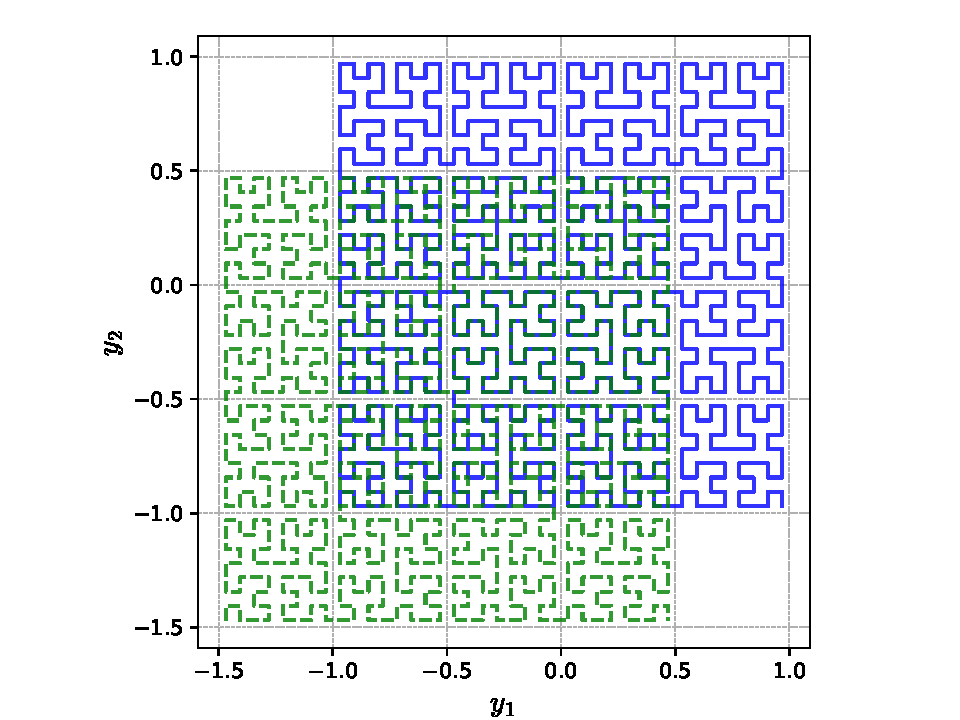
\includegraphics[width=.5\textwidth]{pictures/shifted.pdf}}\label{fig:shifted_ev}}
    %\subfloat[Hypercubes $D_l$]{{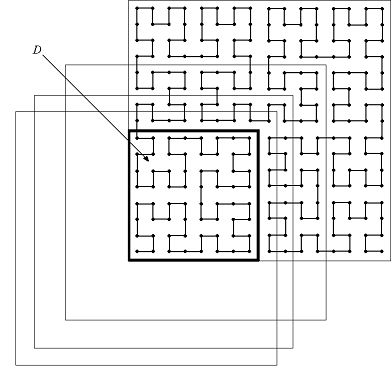
\includegraphics[width=.4\textwidth]{pictures/shifted_cube.png}}\label{fig:shifted_cube}}
    \subfloat[Two rotated evolvents on the same plane]{{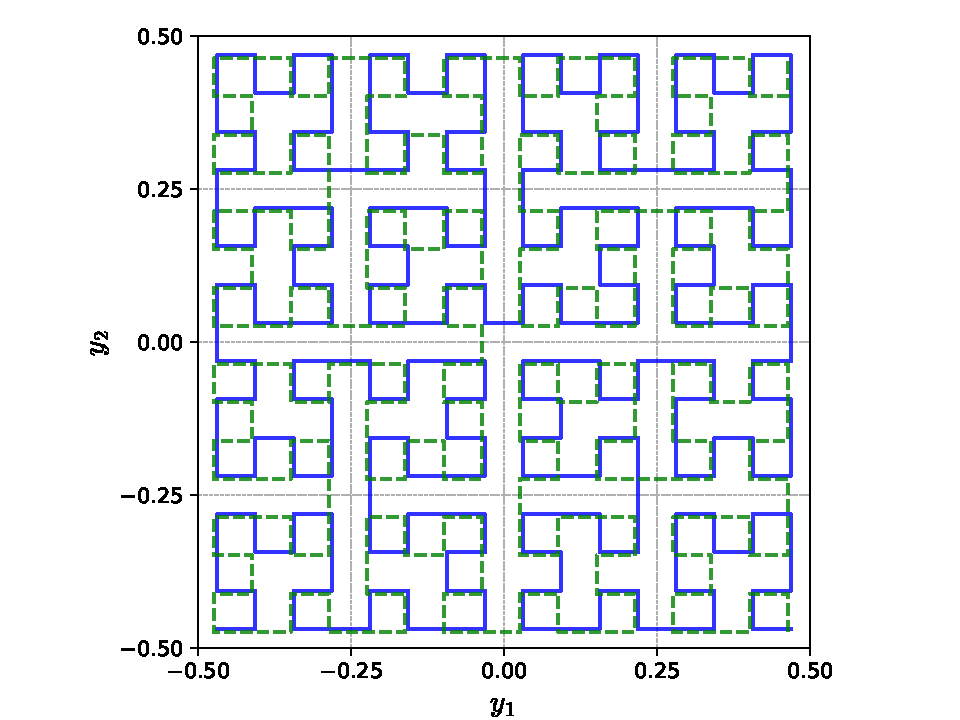
\includegraphics[width=.5\textwidth]{pictures/rotated.pdf}}\label{6_fig_9}}
    \caption{Multiple evolvents built with low density }
\end{figure}

%------------------------------------------------------------------------------
\subsection{Rotated evolvents}
The application of the scheme for building the multiple evolvents (hereinafter called the shifted
evolvents or $S$-evolvents) described in Subsection \ref{sec:shifted} allows to preserve the
information on the nearness of the points in the multidimensional space and, therefore, to
provide more precise (as compared to a single evolvent) estimate of Lipschitz constant in the
search process. However, this approach has serious restrictions, which narrow the applicability
of the parallel algorithms, designed on the base of the $S$-evolvents (see the end of the section
\ref{sec:seq_comp}).

To overcome complexity of the $S$-evolvent and to preserve the information on the nearness of the points in
the $N$-dimensional space, one more scheme of building of the multiple mappings was proposed.
The building of a set of Peano curves not by the shift along the main diagonal of the hypercube
but by rotation of the evolvents around the coordinate origin is a distinctive feature of the
proposed scheme \cite{Gergel2009}.
In Fig.~\ref{6_fig_9} two evolvents being the approximations to Peano curves for the case
$N=2$ are presented as an illustration.
Taking into account the initial mapping, one can conclude that current implementation of the
method allows to build up to $N(N-1)+1$ evolvents for mapping the $N$-dimensional domain
onto the corresponding one-dimensional intervals. Moreover, the additional constraint  $g_0(y)
\leq 0$ with $g_0(y)$ from (\ref{6_g0}), which arises in shifted evolvents, is absent. This
method for building a set of mappings can be ``scaled'' easily to obtain more evolvents (up to
$2^N$) if necessary.

%\begin{figure}[t]
%  \centering
%  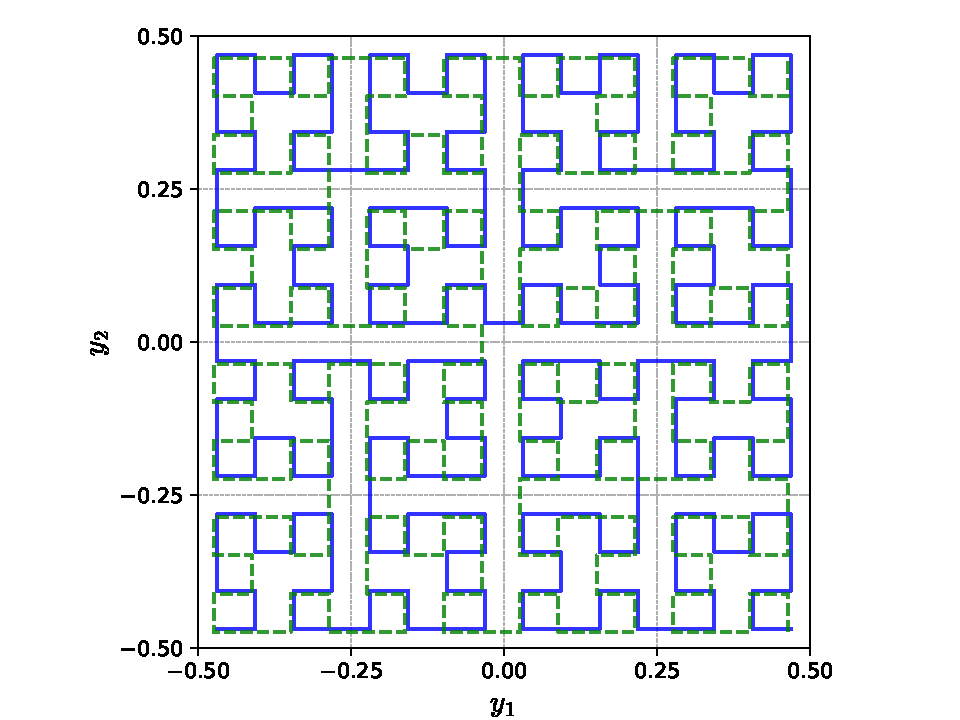
\includegraphics[width=0.6\linewidth]{pictures/rotated.pdf}
%  \caption{Two rotated evolvents on the same plane}
%  \label{6_fig_9}
%\end{figure}

%------------------------------------------------------------------------------
\subsection{Non-Univalent evolvent}

As it has been already mentioned above (Sec.~\ref{sec:shifted}), the loss of information on the
proximity of the points in the multidimensional space could be compensated in part by the use
of multiple mappings $Y_L(x)=\{y^1(x),...,y^L(x)\}$. However, the Peano-type curve preserves
a part of this information itself: it is not an injective mapping. Therefore, if a single image
$y(x)\in \mathbb{R}^N$ is available, on can obtain several different preimages
$t_j\in[0,1], t_j \not = x$, which could be added into the search information of the method later.

The Peano-type curve used in (\ref{eq:oneDimTask}) for the dimensionality reduction is
defined via the transition to the limit. Therefore, it cannot be computed directly. In the
numerical optimization, some approximation of this curve is used, and it is an injective piecewise-linear curve. In \cite{strongin1978} a non-univalent mapping of a uniform grid in the
interval $[0,1]$ onto a uniform grid in a hypercube $D$ has been proposed. Each
multidimensional node can have up to $2^N$ one-dimensional preimages. In
Fig.~\ref{fig:noninjective}, the grid in the $\mathbb{R}^2$ space is marked by the crosses, for
two nodes of which the corresponding one-dimensional preimages from $[0,1]$ are pointed
(marked by the squares and circles). Each node mentioned above has 3 preimages.

A potentially large number of preimages (up to $2^N$) and the inability to use the parallel
scheme for the multiple mappings are the disadvantages of the non-univalent evolvent.

%------------------------------------------------------------------------------
\subsection{Smooth evolvent}

The methods of constructing the evolvents considered in the previous paragraphs produce the
curve $y(x)$, which in not a smooth one (see Fig.~\ref{fig:shifted_ev}). The absence of
smoothness may affect the properties of the reduced one-dimensional function $\varphi(y(x))$
adversely since a smooth curve reflect the information on the growth/decay of the initial
function better. On the basis of initial algorithm of constructing the non-smooth evolvent, a
generalized algorithm allowing constructing a smooth space-filling curve has been
proposed~\cite{Goryachih2017}. As an illustration, a smooth evolvent for the two-dimensional
case is presented in Fig.~\ref{fig:smooth}.
An increased computational complexity (several times as compared to the piecewise-linear
curves) is a disadvantage of the smooth evolvent. This caused by computing of the nonlinear smooth
functions.
%At that, the number of smooth intervals and the difficulty of the
%computations of the curve increases with increasing accuracy of approximation and
%space dimension.

\begin{figure}[ht]
    \centering
    \subfloat[Smooth evolvent]{{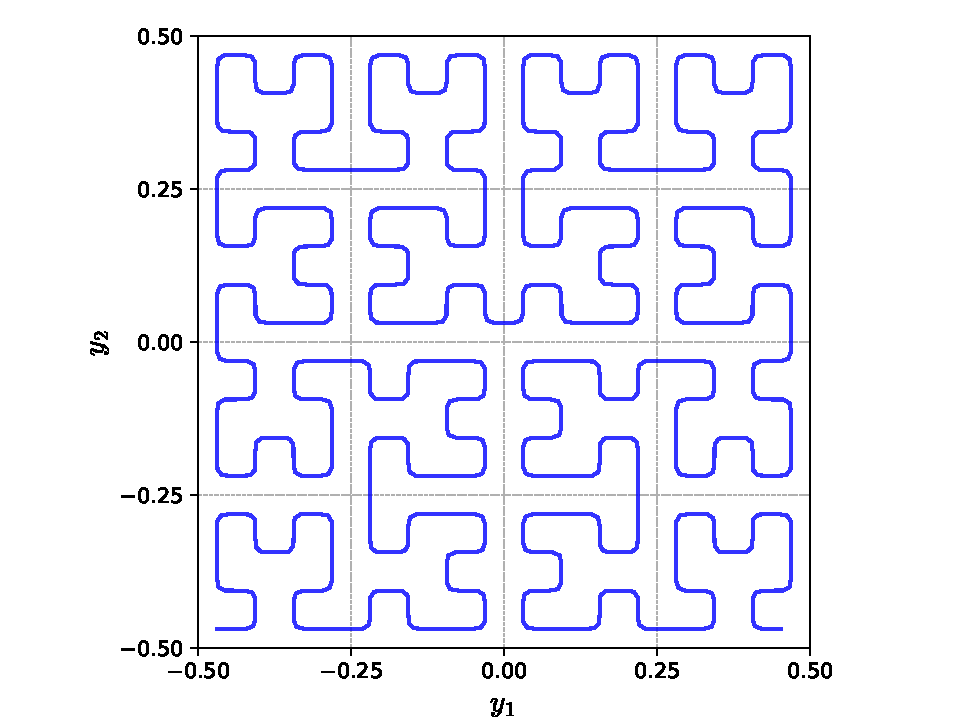
\includegraphics[width=.6\textwidth]{pictures/smooth.pdf}}\label{fig:smooth}}
    \subfloat[Non-univalent
evolvent]{{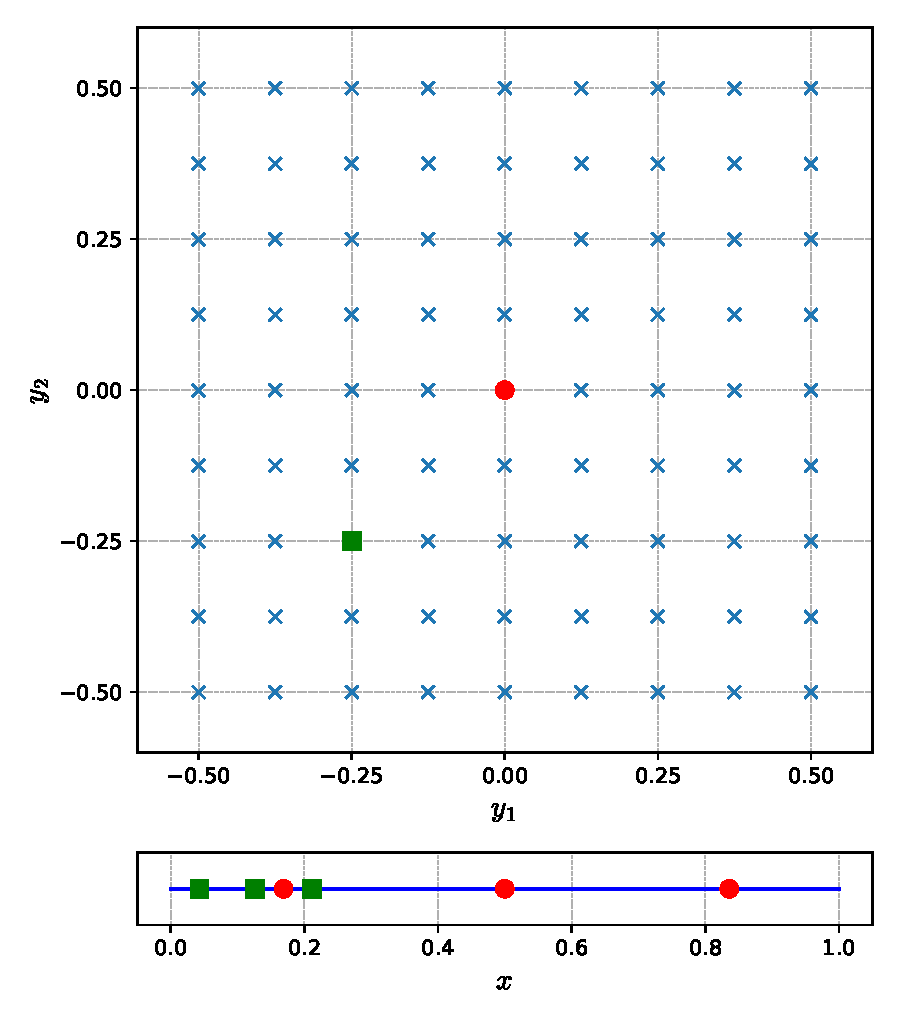
\includegraphics[width=.4\textwidth]{pictures/noninjective.pdf}}\label{fig:noninjective}}
    \caption{Different evolvents built with low density}
\end{figure}

\section{Core Multidimensional Algorithm of Global Search}

The optimization methods applied in Globalizer to solve the reduced problem
(\ref{eq:oneDimTask}) are based on the MAGS method, which can be presented as follows ---
see \cite{strongin1978}, \cite{strSergGO}.
\par
The initial iteration of the algorithm is performed at an arbitrary point \mbox{\(x^1\in(0,1)\)}.
Then, let us suppose that \(k\), \(k\ge 1\), optimization iterations have been completed already.
The selection of the trial point \(x^{k+1}\) for the next iteration is performed according to the
following rules.

\textit{Rule 1}. Renumber the points of the preceding trials by the lower indices in order of
increasing value of coordinates
$0=x_0<x_1<...<x_{k+1}=1$.

\textit{Rule 2}. Compute the characteristics \(R(i)\) for each interval \((x_{i-1},x_i),1\leq i\leq
k+1\).

\textit{Rule 4}. Determine the interval with the maximum characteristic $R(t)=\max_{1\leq i
\leq k+1}R(i)$.

\textit{Rule 5}. Execute a new trial at the point \(x^{k+1}\) located within the interval with the
maximum characteristic from the previous step
  $x^{k+1}=d(x_t)$.

The stopping condition, which terminated the trials, is defined by the inequality
$\rho_t<\varepsilon$
for the interval with the maximum characteristic from Step 4 and \(\varepsilon >0\) is the
predefined
accuracy of the optimization problem solution. If the stopping condition is not satisfied,
the index \(k\) is incremented by 1, and the new global optimization iteration is executed.

The convergence conditions and exact formulas for decision rules $R(i)$ and $d(x)$ of the
described algorithm are given, for example, in \cite{strSergGO}.

%------------------------------------------------------------------------------
\section{Results of Numerical Experiments}
%\begin{Russian}

The computational experiments have been carried out on the Lobachevsky supercomputer at
State University of Nizhni Novgorod. A computational node included 2 Intel
Sandy Bridge E5-2660 2.2 GHz processors, 64 GB RAM. The CPUs had 8 cores (i. e. total 16
cores were available per a node). All considered algorithms and evolvents were implemented
using C++ within the Globalizer software system~\cite{globalizerSystem}.

The comparison of the global optimization algorithms was performed by the evaluation of the
quality of solving a set of problems from some test class.
In the present paper, the test class generated by GKLS generator~\cite{Gaviano2003} was
considered. This generator allows constructing the complex multiextremal problems of various
dimensions. In the present work, the series of 100 problems from the classes of the dimensions
of 2, 3, 4, and 5 were considered.
Each class had two degrees of complexity --- \textit{Simple} and \textit{Hard}. The parameters
of the generator for the considered classes were given in Ref.~\cite{Gaviano2003}.

In order to evaluate the efficiency of an algorithm on a given set of 100 problems, we will use
the operating characteristics \cite{grishaginClass}, which are defined as a
curve, showing the dependency of number of solved problems vs the number of iterations.

%------------------------------------------------------------------------------
\subsection{Comparison of the sequential evolvents}
\label{sec:seq_comp}
%\begin{Russian}
In order to understand whether any type of evolvents listed above has an essential advantage as
compared to other ones, the operating characteristics of the index method with different types
of evolvents have been obtained for the classes GKLS 2d Simple and GKLS 3d Simple. The
global minimum was considered to be found if the algorithm generates a trial point $y^k$ in the
$\delta$-vicinity of the global minimizer, i.e. $\left\|y^k-y^\ast\right\|_\infty\leq\delta$. The size
of the vicinity was selected as $\delta = 0.01\left\|b-a\right\|_\infty$. In case of GKLS
$\delta=0.01$.

In all experiments, the evolvent construction density parameter $m=12$. The minimum value of
the reliability parameter \(r\) was found for each type of evolvents by scanning over a uniform grid
with the step \(0.1\).

On the GKLS 2d Simple class at the minimum \(r\), the non-univalent evolvent and the smooth
one provide a faster convergence (Fig.~\ref{fig:gkls2d_opt}). The same was observed at
\(r=5.0\) as well (Fig.~\ref{fig:gkls2d_acc}). In the latter case, the shifted evolvent and the
rotating one begin to lag behind the rest since the value \(r=5.0\) is too big for them.
\begin{figure}[ht]
    \centering

\subfloat[$r=5.0$]{{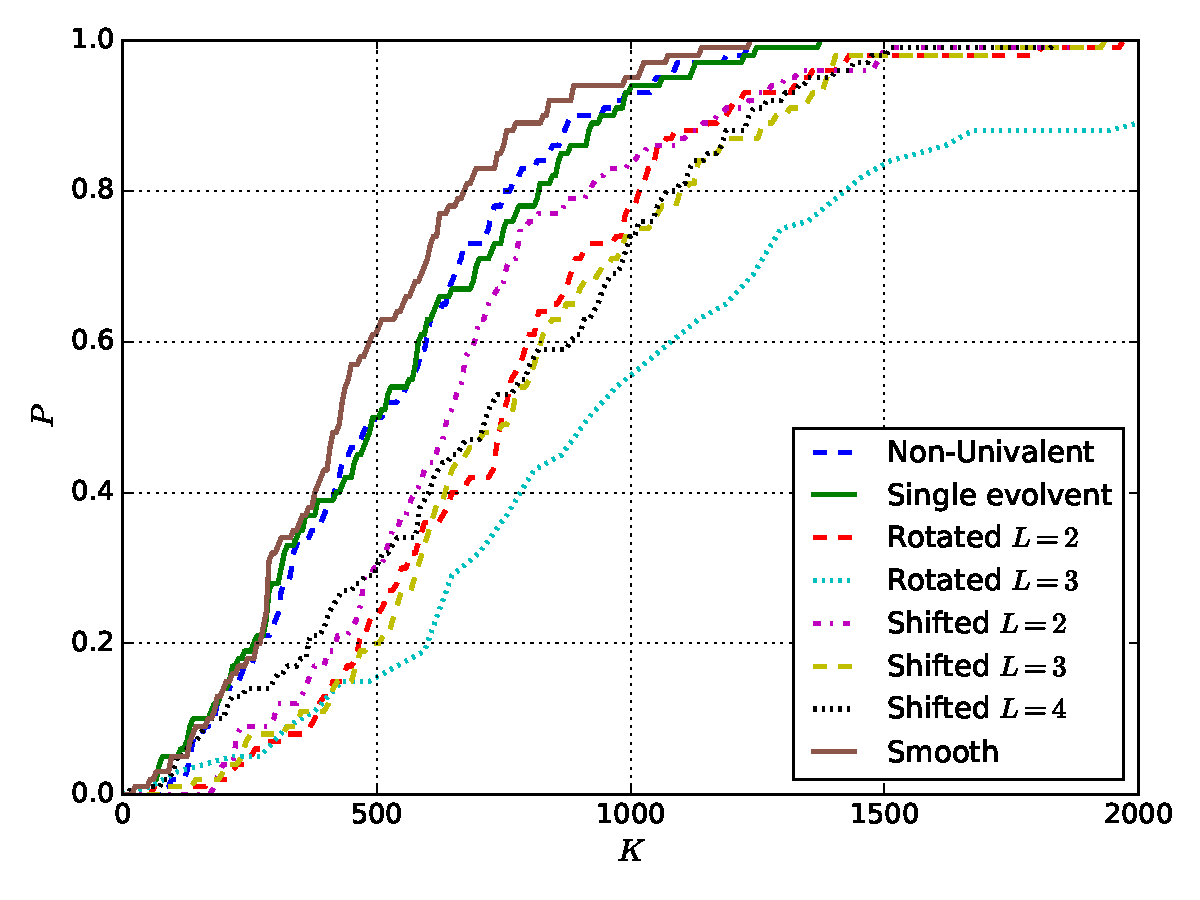
\includegraphics[width=.5\textwidth]{pictures/gklsS2d_same_r_opt_pt_op.pdf}}\label{fig:gkls2d_acc}}
    \subfloat[Minimal
$r$]{{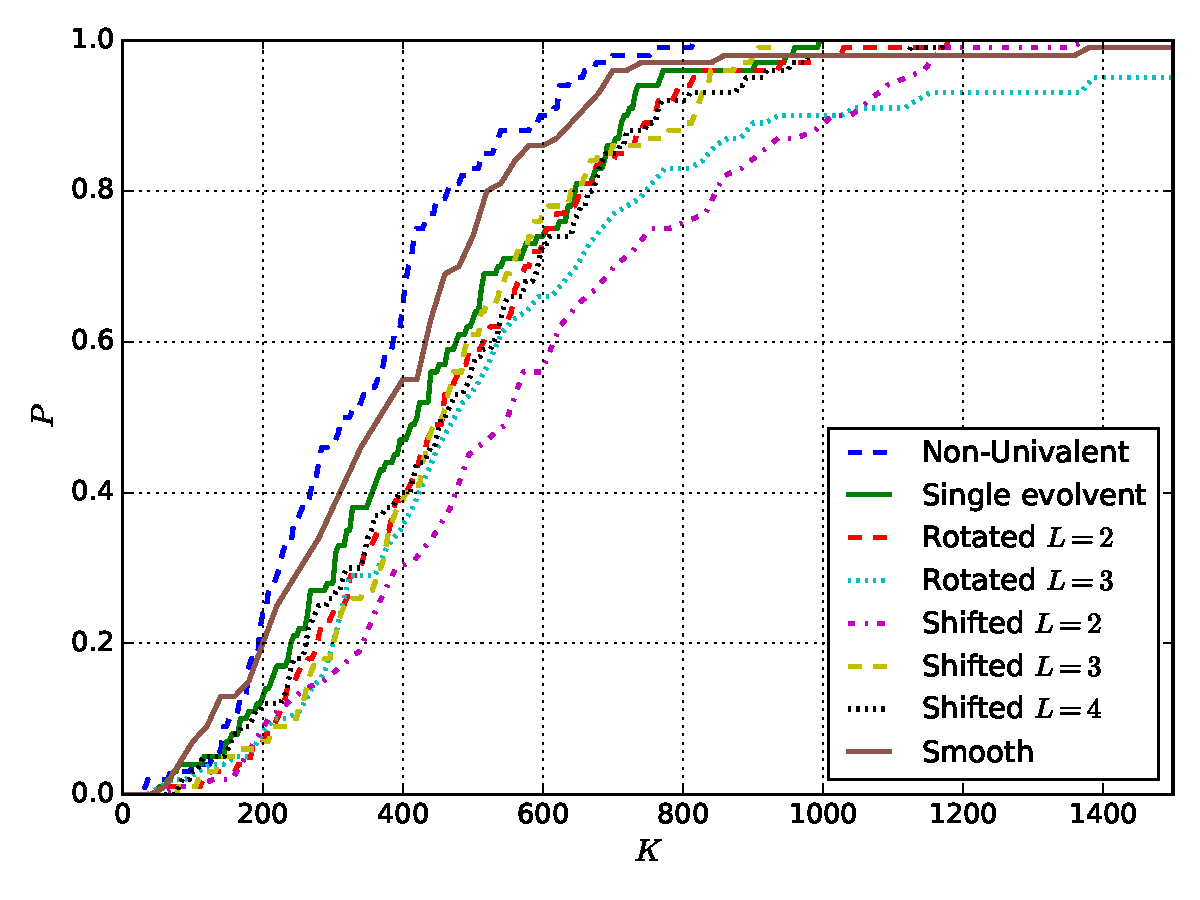
\includegraphics[width=.5\textwidth]{pictures/gklsS2d_opt_pt_op.pdf}}\label{fig:gkls2d_opt}}
    \caption{Operating characteristics on GKLS 2d Simple class}
\end{figure}

On the GKLS 2d Simple class at the minimum \(r\), the non-univalent evolvents and multiple
ones have a considerable advantage over the single evolvent (Fig.~\ref{fig:gkls3d_opt}).
The value \(r=4.5\) is too big for the rotated evolvents and for the shifted one
(Fig.~\ref{fig:gkls3d_acc}).

\begin{figure}[ht]
    \centering

\subfloat[$r=4.5$]{{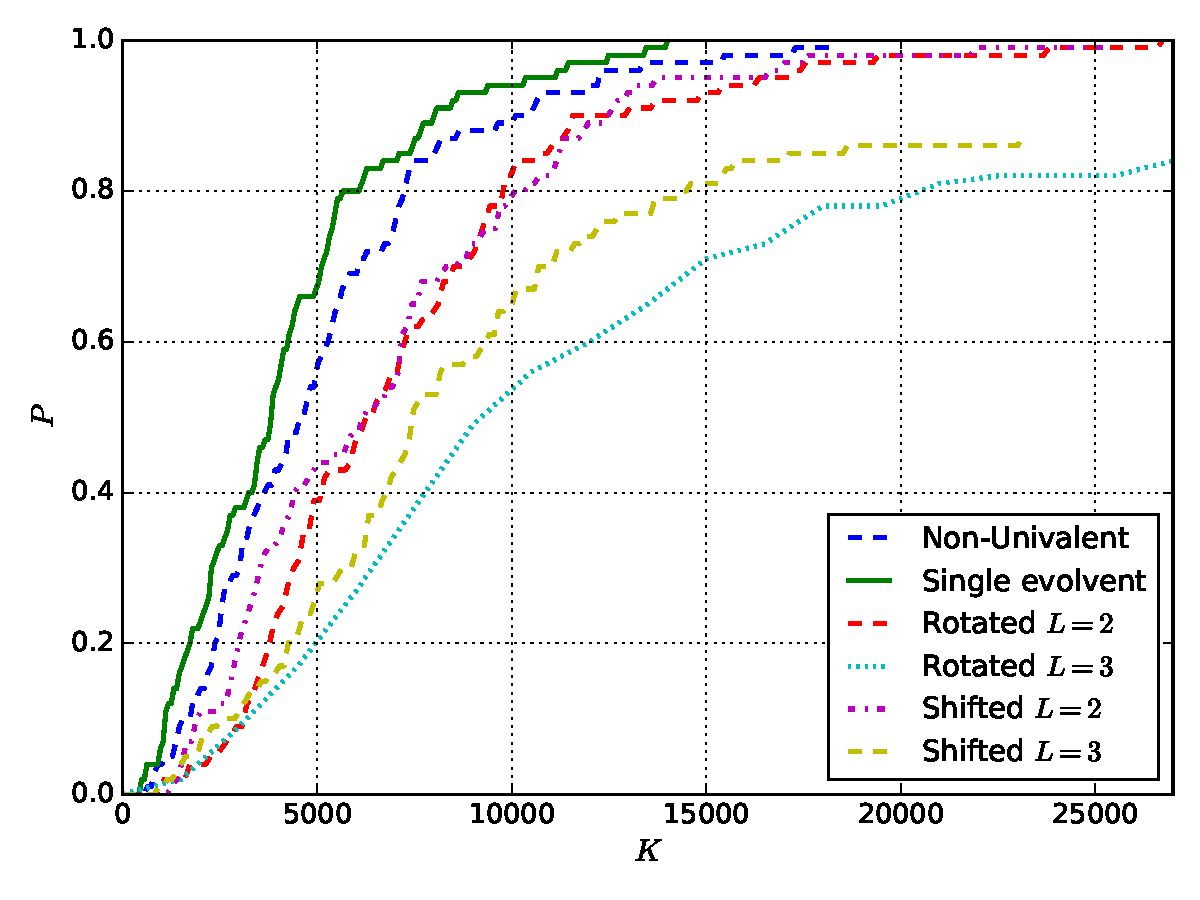
\includegraphics[width=.5\textwidth]{pictures/gklsS3d_same_r_opt_pt_op.pdf}}\label{fig:gkls3d_acc}}
    \subfloat[Minimal
$r$]{{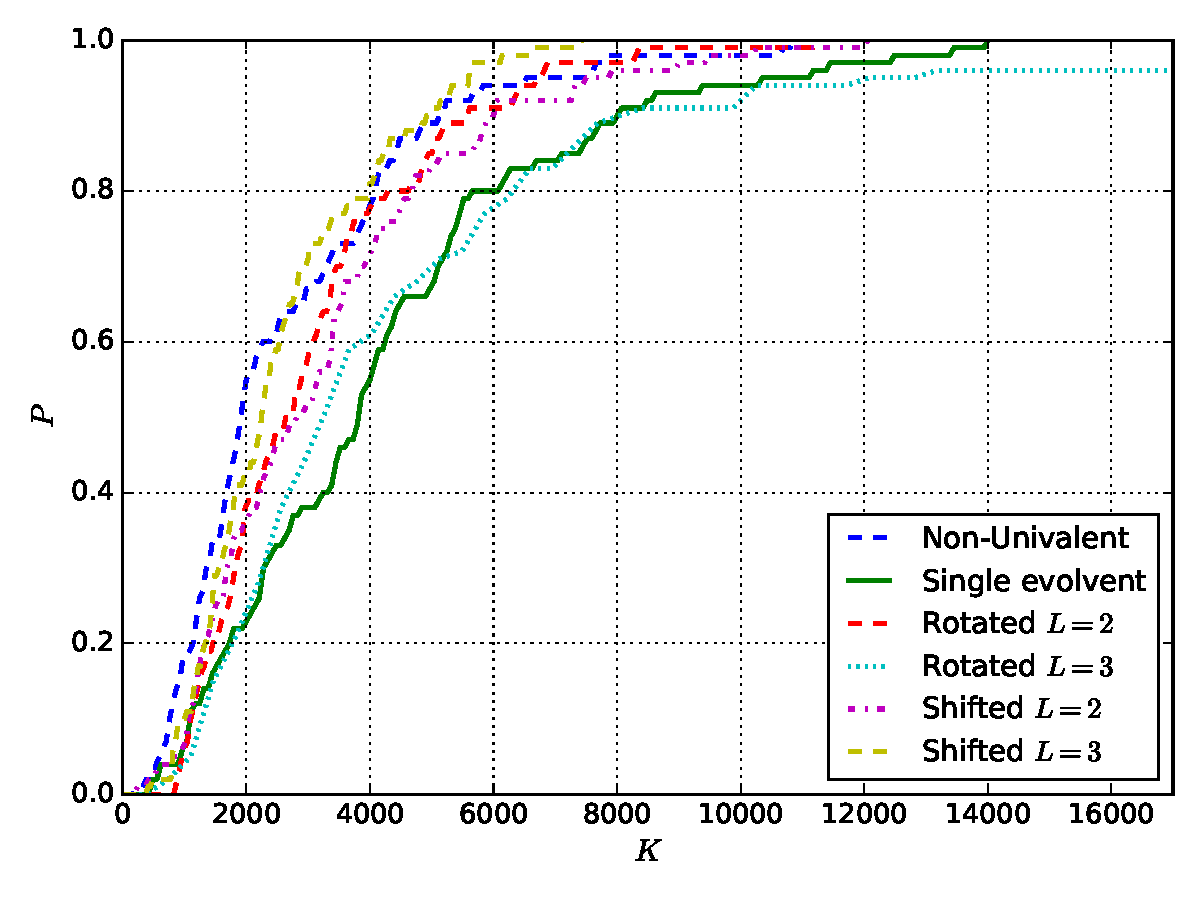
\includegraphics[width=.5\textwidth]{pictures/gklsS3d_opt_pt_op.pdf}}\label{fig:gkls3d_opt}}
    \caption{Operating characteristics on GKLS 3d Simple class}
\end{figure}

\paragraph{Overhead costs when using the shifted evolvents.}
In all experiments presented above, the number of computations of the objective function from
the GKLS class was taken into account when plotting the operating characteristics. However, in
the case of the shifted evolvent, the index method solves the problem with the constraint \(g_0\)
from (\ref{6_g0}). At the points where \(g_0\) is violated, the value of the objective function is
not computed. Nevertheless, these points are stored in the search information producing the
additional computational costs. In Table~\ref{tab:shifted_g0}, the averaged numbers of calls to
\(g_0\) and to the objective function are presented. At \(L=3\), the constraint \(g_0\) was
computed almost 20 times more than the objective function \(\varphi\) i. e. \(95\%\) of the whole
search information account for the auxiliary points. Such overhead costs are acceptable when
solving the problems of small dimension with the computation costly objective functions.
However, when increasing dimensionality and total number of trials other types of evolvents are
preferred.

\begin{table}
\begin{center}
\caption{Averaged number of computations of \(g_0\) and of \(\varphi\) when solving the
problems from GKLS 3d Simple class using the shifted evolvent}
  \begin{tabular}{|l|{c}|{c}|{c}|}
    \hline
  $L$ & $calc(g_0)$ & $calc(\varphi)$ & $\frac{calc(g_0)}{calc(\varphi)}$ ratio \\
  \hline
  2 & 96247.9  & 6840.14 & 14.07\\
  \hline
  3 & 153131.0 & 7702.82 & 19.88\\
  \hline
  \end{tabular}
  \label{tab:shifted_g0}
\end{center}
\end{table}

%------------------------------------------------------------------------------
\section{Conclusions}
In the present work, 5 different Peano curve-type mappings applied to the dimensionality
reduction in the global optimization problems were considered.
From the preliminary comparison conducted in Sec.~\ref{sec:seq_comp}, one can make the
following conclusions:
\begin{itemize}
  \item the smooth evolvent and the non-univalent one demonstrate the best result in the
problems of small dimensionality and can be applied successfully in solving the problems with
the computational costly objective functions. The properties of these evolvents doesn't allow
developing the optimization algorithms scalable onto several cluster nodes based on these ones.
  \item the shifted evolvents introduce large overhead costs on the operation of the method due
to the requirement to adding an auxiliary functional constraint into the problem (\ref{eq:task}).
The experiments have demonstrated that up to 95\% of the search information account for the
points, in which the auxiliary constraint is computed only.
However, if the objective function is computation-costly enough, the use of these evolvents
could make sense.
  \item the rotated evolvents have provided an acceptable speed of convergence in the problems
of small dimensionality in the sequential mode. The use of these ones doesn't result in the
introduction of the auxiliary constraints that allows constructing an efficient parallel algorithm
based on these evolvents.
\end{itemize}

%------------------------------------------------------------------------------
% Index
%\printindex
%\label{sect:bib}
\bibliographystyle{unsrt}
\bibliography{ysc_paper}

%------------------------------------------------------------------------------
\end{document}

% EOF
